%-------------------------------------------------------------------------------
%	CAPITOLO 21
%-------------------------------------------------------------------------------

\chapter{Uno spuntino}
Il povero cav. \index[Personaggi]{Zaccaria Antonio}Antonio Zaccaria, faentino, ispettore della scuola, persona compitissima\footnote{Ben educata, gentile e discreta}, impeccabilmente vestito di nero, barba bianca, alto, compreso della sua missione, moralissimo più realista del Re, un vero tipo e modello di funzionario. Questo l'uomo.\\
\indent Un giorno usciva dalla scuola del \index[Luoghi]{Borgo Gallina}Borgo Gallina\footnote{Detto anche Borgo Fratti, è la zona a ridosso del fiume in vi Antonio Fratti}, sul mezzogiorno, incontra una vecchietta, con affabilità, sottovoce e gran circospezione, le dice: <<Buona donna, spendendo poco si potrebbe fare uno spuntino?>>.\\
\indent La vecchia, sorpresa dal fare circospetto e misterioso del cavaliere, e molto a digiuno della lingua di Dante, inarca le ciglia, si mette le mani sulla cintola e come suol dire si inalbera ed acerba risponde: <<Cossa, me a so vecia, mo d'al cos che l'è an no mai fat e mai aiò tnu man...\footnote{<<Cosa? Io sono vecchia, ma delle cose come quella non ne ho mai fatte e mai ne ho tenuto mano!>>}>>.\\
\indent Il povero ispettore allibì, temendo di sollevare uno scandalo per l'ignoranza della vecchia, si riprese ed affascinante rispose: <<Oh! Oh! Buona donna che cosa avete mai capito! Voglio dire se si possono mangiare due ova al tegame!>>\\
\indent La vecchia, schiarita nelle idee e nella faccia, replicò: <<Mo alora u m'à da dì che vò magné!\footnote{<<Ma allora mi deve dire che vuol mangiare!>>}>>\\
\indent E le cose si accodarono tra la vecchia e il cavaliere.

 \begin{figure}[htb]
    \centering
    %\vspace{-0.7cm}
    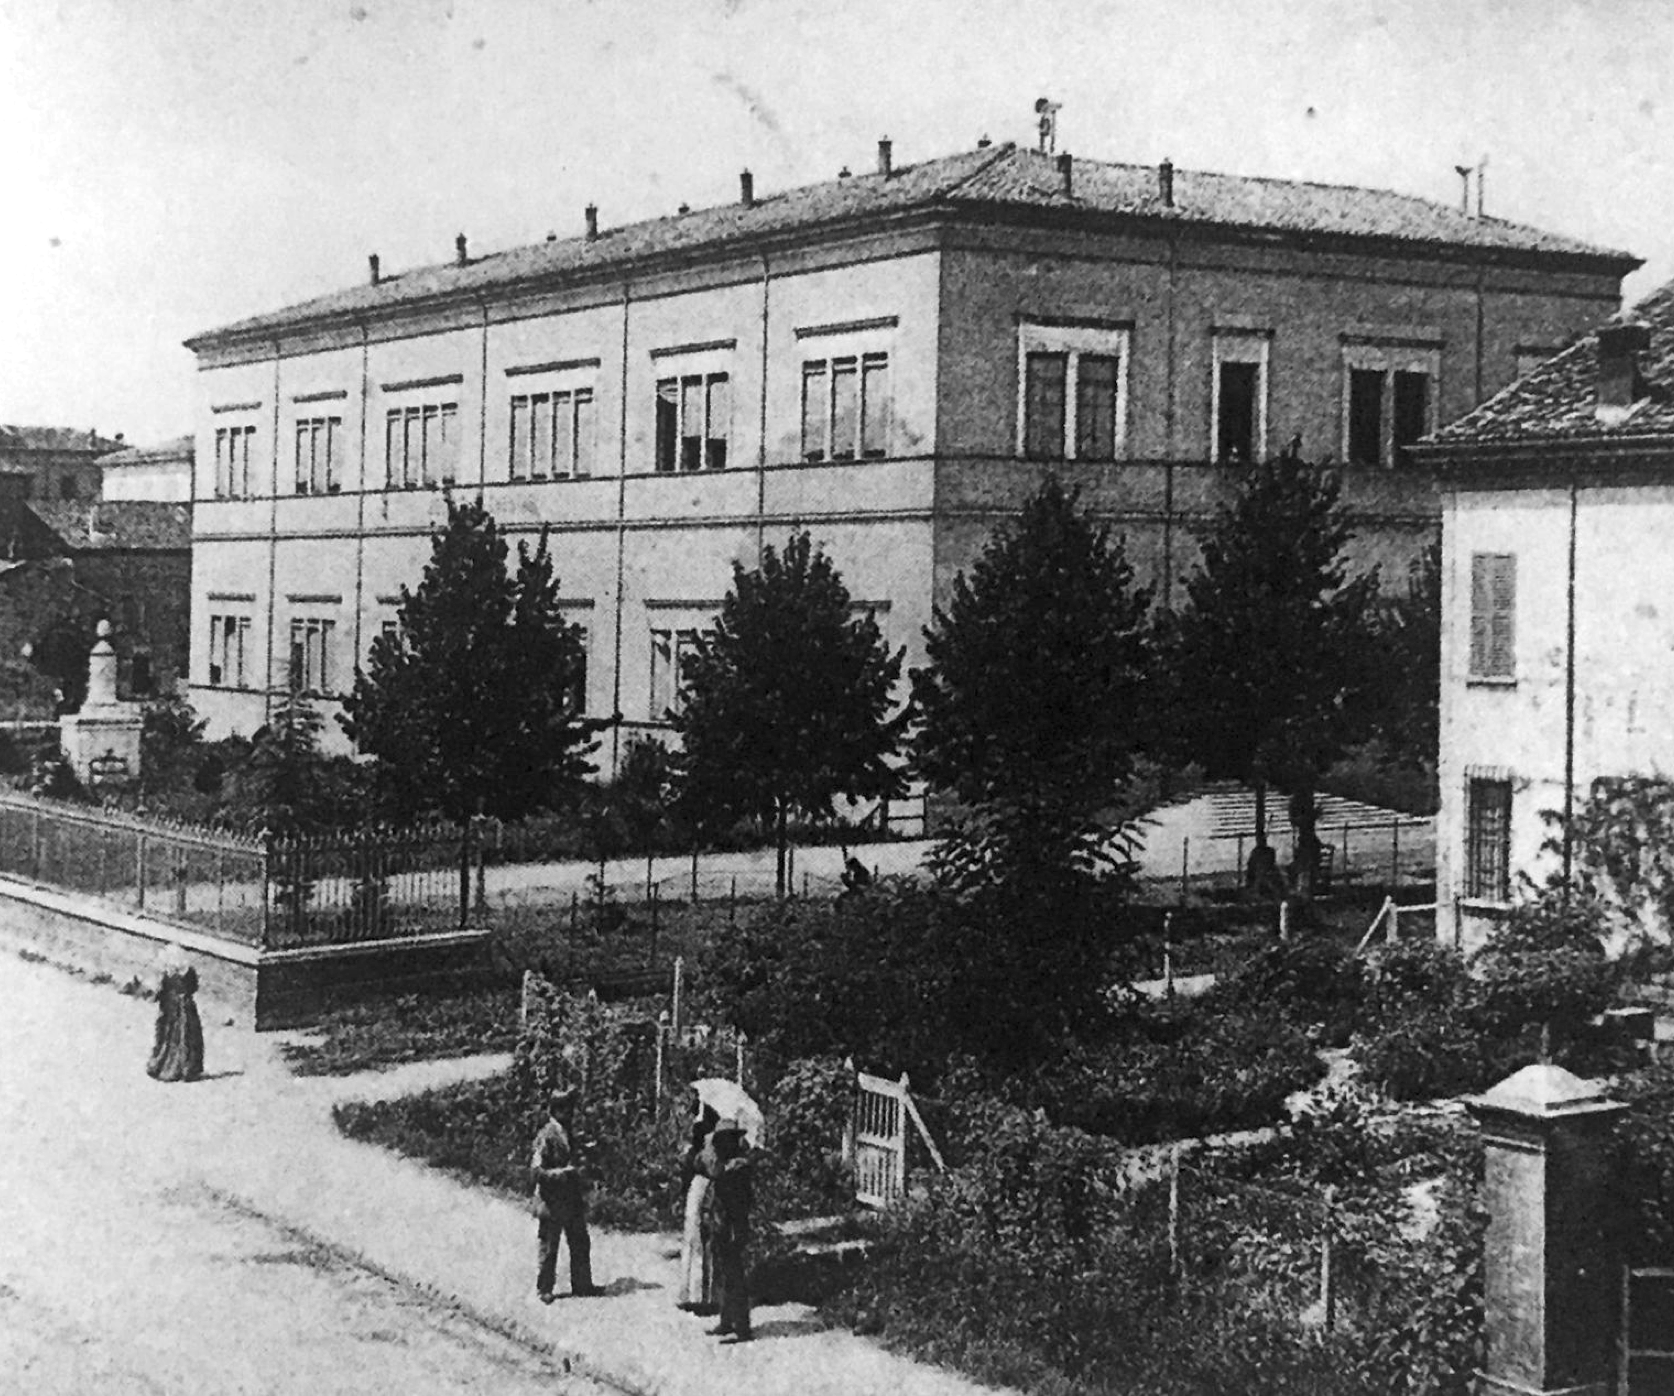
\includegraphics[width=\textwidth]{scuole}
    \caption[Scuole Comunali]{Le scuole comunali di Alfonsine, in Corso Garibaldi. Si può osservare sulla sinistra il monumento della Pigna che attualmente è nel parchetto di fronte alla Chiesa Sacro Cuore.\label{fig:scuole}}
    %\vspace{-0.3cm}
\end{figure}